Das \ac{http} ist ein Protokoll das in der Internet-Kommunikation zum Einsatz kommt.
Es dient zur Übertragung von Daten zwischen einem Client und einem Server und wird hauptsächlich zur Auslieferung beziehungsweise Bedienung von Webanwendungen genutzt.
Seit der Einführung in 1991 wurde es in mehreren RFCs erweitert und ist inzwischen in Version drei\cite{onlineIETFErhebtHTTP2022}.\\

Das der \ac{http}-Kommunikation zu Grunde liegende Interaktionsmuster erfolgt nach den \textit{Request-Response-Pattern}.
Ein Client beginnt die Kommunikation und fragt Daten oder Daten-Operationen an einem Server an.
Der Server beantwortet diese Anfrage\footnote{Im folgenden werden \ac{http}-Anfrage und das Englische \ac{http}-Request synonym verwendet. Das Gleiche gilt für \ac{http}-Antwort und \ac{http}-Response} und sendet dem Client Informationen wie die Verarbeitung erfolgt ist und die Angeforderten Daten.
Diese Kommunikation erfolgt über TCP.
Ist ein Request-Response Cycle abgeschlossen, wird die TCP-Verbindung gekappt und der Server kann keine weiteren Nachrichten an den Client schicken bis dieser eine neue Anfrage startet.
Übertragen werden können Texte in diversen Formatierungen wie beispielsweise H\textit{TML-Dokument} oder \textit{JSON-Strings}, es ist jedoch auch möglich Binär-Daten wie \textit{Bilddateien} zu übertragen.
HTML ist ein \textit{Plaintext}-Protokoll, die Kommunikation erfolgt unverschlüsselt.
Außerdem ist \ac{http} Textbasiert, eine Nachricht wird in Textform übertragen und ist menschenlesbar.

Die oben beschrieben Eigenschaften beziehen sich auf \ac{http} in Version 1.
Seit dieser Version wurden einige Erweiterungen an \ac{http} vorgenommen, hauptsächlich mit dem Ziel die Kommunikationsgeschwindigkeit des Protokolls zu erhöhen.
So kann TCP-Pipelining genutzt werden um mehrere TCP-Nachrichten nacheinander zu schicken ohne Bestätigung des Erhaltens der Nachricht abzuwarten.
Außerdem werden Push-Nachrichten unterstützt:
Der Server kann durch Aufrechterhaltung einer TCP-Verbindung weitere \ac{http}-Nachrichten an den Client schicken.
Mit Version 3 wurde \ac{http} Außerdem auf das Stream-basierte QUIC Protokoll umgestellt um die Kommunikation weiter zu Optimieren\cite{OverviewHTTPHTTP2023}.\\

Da die grundlegenden Funktion von \ac{http} 1.0 und 1.1 ausreichend ist um eine \ac{waf} zu erklären, wird im Folgenden nur diese betrachtet.

\paragraph{\ac{http}-Nachrichten \cite{HTTPMessagesHTTP2024}}
\ \\
Die Grundlegende Einheit einer \ac{http}-Kommunikation wird als \textit{Nachricht} bezeichnet.
Da \ac{http} ein Klartext-Protokoll ist, werden diese in menschenlesbarer Form als Text übertragen.
Eine Nachricht besteht aus einer \textit{Start-Zeile}, die die Nachricht entweder als Anfrage oder Antwort identifiziert.
In den beiden Fälle ist der Aufbau dieser Zeile unterschiedlich:

\begin{figure}[!hbt]
     \centering
     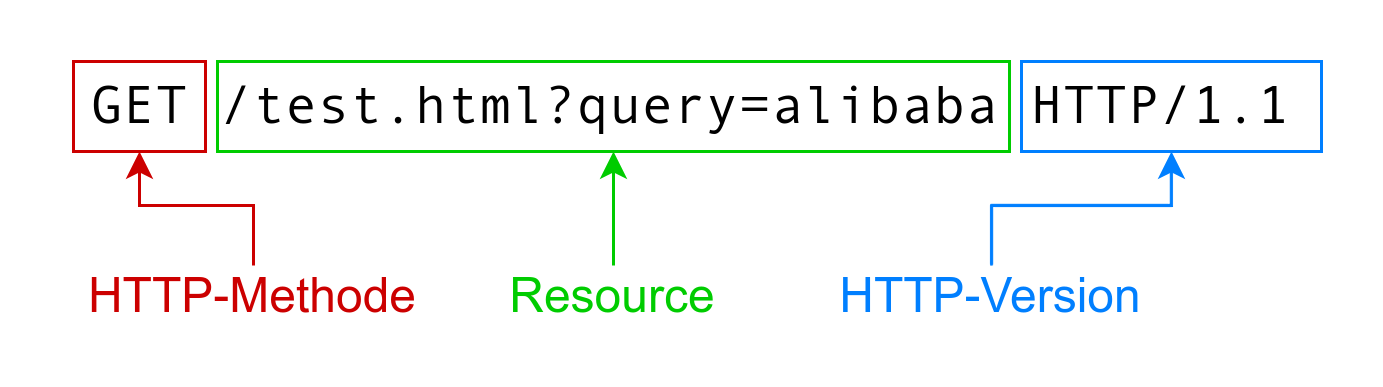
\includegraphics[width=0.9\textwidth]{./images/HTTP-Requestline.png}
     \caption{Beispiel für eine \ac{http} Request-Zeile}
     \floatfoot{Quelle: Eigene Darstellung}
     \label{fig:http-requestline}
 \end{figure}

\begin{description}
     \item[Request-Zeile:] Ein \ac{http}-Request ist durch eine \textit{Request-Zeile} identifiziert. Diese ist in drei Teile aufgeteilt (siehe Abbildung \ref{fig:http-requestline}).
     \begin{description}
          \item[Die \ac{http}-Methode] beschreibt die Operation, die der Server ausführen soll.
          Die Operationsbezeichner können auch \textit{\ac{http}-Verben} und \textit{\ac{http}-Nomen} genannt werden.
          Syntaktisch basieren die Methoden auf dem FTP Protokoll, das älter ist und mit Operationen wie GET und PUT arbeitet.
          In höheren Versionen wird der Satz an Verben und Nomen jedoch um weitere Methoden, wie zum Beispiel PATCH oder OPTIONS, erweitert.
          \item[Die Resource] beschreibt das angefragte Objekt, üblicherweise in einer \ac{url}. 
          Optional kann die angefragte Resource mit einem Fragezeichen gefolgt von einem sogenannten \textit{Query String} noch spezifiziert beziehungsweise gefiltert werden.
          \item[Die \ac{http} Version] die angibt in welcher Version die folgende Nachricht verfasst ist. 
     \end{description}
\end{description}

\begin{figure}[!hbt]
     \centering
     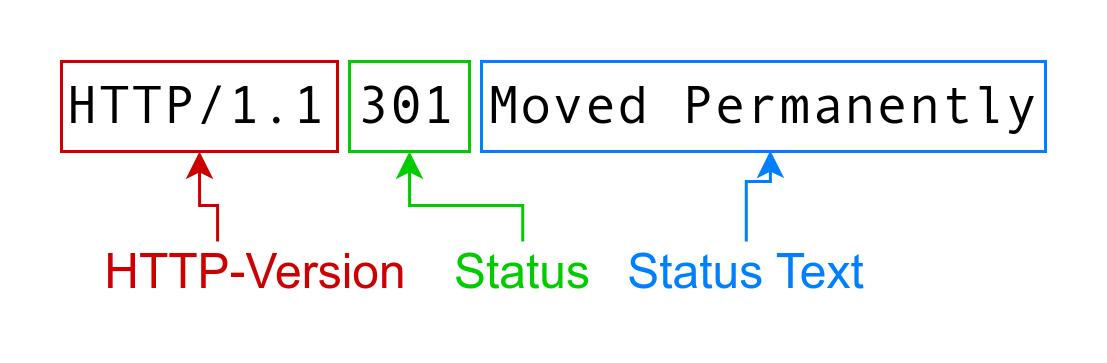
\includegraphics[width=0.9\textwidth]{./images/HTTP-Statusline.png}
     \caption{Beispiel für eine \ac{http} Status-Zeile}
     \floatfoot{Quelle: Eigene Darstellung}
     \label{fig:http-statusline}
 \end{figure}


\begin{description}
     \item[Status-Zeile:] Die Antwort auf einen Request beginnt mit einer Status-Zeile in einem eigenen Format, die wie die Request-Zeile aus drei Teilen besteht (siehe Abb. \ref{fig:http-statusline}).
     \begin{description}
          \item[Die \ac{http} Version] gibt, wie an dritter Stelle des \ac{http}-Requests, die \ac{http}-Version der Folgenden Nachricht an.
          \item[Der Status Code] der durch einen dreistelligen Zahlencode angibt wie der Status der Verarbeitung eines Requests ist. 
          Die erste Stelle Signalisiert grob von welcher Art das Ergebnis ist. 
          So steht zum Beispiel 2xx für eine Erfolgreiche Verarbeitung während 4xx auf einen Fehler auf Client-Seite hindeutet.
          Die zwei folgenden Stellen geben genauer Aufschluss wie der Status ist\cite{HTTPResponseStatus2023}.
          \item[Der Status Text] ist ein Beliebiger Text der den Status genauer beschreibt.
          Im \ac{http} Standard ist zwar nicht vorgeschrieben wie der Text auszusehen hat, es gibt jedoch Konventionen\cite{HTTPResponseStatus2023}.
     \end{description}
\end{description}

Nach der Start-Zeile folgen sowohl in einem \ac{http}-Request als auch in der Response zwei weitere Abschnitte. 
Diese werden genutzt, um der Nachricht weitere Informationen hinzuzufügen.

Die \textbf{\ac{http}-Header} sind Key-Value Pare. Der Key ist ein \textit{case sensitiver} String.
Der Value ist beliebig darf jedoch keinen Zeilenumbruch enthalten, da dies den Beginn eines neuen Header Key-Value-Pares anzeigt.
Die Header teilen sich in unterkategorien wie \textit{Request-} oder \textit{General-Header} auf, an diesem Punkt ist es im Rahmen dieser Thesis jedoch nicht notwendig weiter in die Tiefe zu gehen.
Eine Relevante Header-Gruppe sind die \textit{Representation-Header}, die die Formatierung des \ac{http}-Bodies genauer spezifizieren.
Hier kann der Datentyp und die Endcodierung des Bodies angegeben werden.

Der \textbf{\ac{http}-Body} enthält die Daten die mit der \ac{http}-Nachricht versendet werden und ist optional
Im Body können sich beliebige Daten befinden: Binärdaten wie Bilder, JSON-Formatierte Strings oder einfacher Text\cite{HTTPMessagesHTTP2024}.\\

Wie oben beschrieben, bietet \ac{http} zahlreiche Möglichkeiten an, einem Server Daten zu übergeben oder von einem solchen Daten zu erhalten.
Alle Felder werden verarbeitet und bieten somit theoretisch die Möglichkeit zur Übermittlung schadhafter Daten.
Auch die Möglichkeit zur codierten Übertragung, speziell im \textit{\ac{http}-Body}, kann zu diversen Angriffsvektoren führen.
Eine \ac{waf} muss in der Lage sein alle dieser Parameter überblicken zu können um effektiven Schutz zu bieten.

\pagebreak    